%\documentclass[preprint,tightenlines,showpacs,showkeys,floatfix,
%nofootinbib,superscriptaddress,fleqn]{revtex4} 
\documentclass[tightenlines,floatfix,nofootinbib,superscriptaddress,fleqn]{revtex4} 
%\documentclass[aps,epsfig,tightlines,fleqn]{revtex4}
\usepackage{kotex}
\usepackage[HWP]{dhucs-interword}
\usepackage[dvips]{color}
\usepackage{graphicx}
\usepackage{bm}
%\usepackage{fancyhdr}
%\usepackage{dcolumn}
\usepackage{defcolor}
\usepackage{amsmath}
\usepackage{amsfonts}
\usepackage{amssymb}
\usepackage{amscd}
\usepackage{amsthm}
\usepackage[utf8]{inputenc}
%\pagestyle{fancy}

\begin{document}

\title{\Large 2022년 2학기 물리학 II}
\author{김현철\footnote{Office: 5S-436D (면담시간 매주
    수요일-16:15$\sim$19:00)}} 
\email{hchkim@inha.ac.kr}
\affiliation{Hadron Theory Group, Department of Physics,
  Inha  University, Incheon 22212, Republic of Korea }
\date{Autumn Semester, 2022}

\maketitle

{\color{red} {\bf Due date:} 2022년 9월 19일  15:30-16:15 }
\vspace{1.cm}

\noindent \textbf{ 주의: \color{blue} 단 한 번의 부정행위도 절대
  용납하지 않습니다. 적발 시, 학점은 F를 받게 됨은 물론이고,
  징계위원회에 회부합니다. One strike out임을 명심하세요.} 
\\
\\

{\bf 학번:} \hspace{4cm}
{\bf 이름:} 

\section*{\large Quiz 6}
\noindent {\bf 문제 1 [20pt].}
그림~\ref{fig:1}처럼 평행판 축전기 한 판의 변의 길이는 각각 $10$
cm이고, 판 사이의 거리는 $d=4.0$ mm이다. 이 축전기에 들어있는 유전
물질의 유전상수는 $\kappa=2.0$이다. 
\begin{figure}[htp]
  \centering
  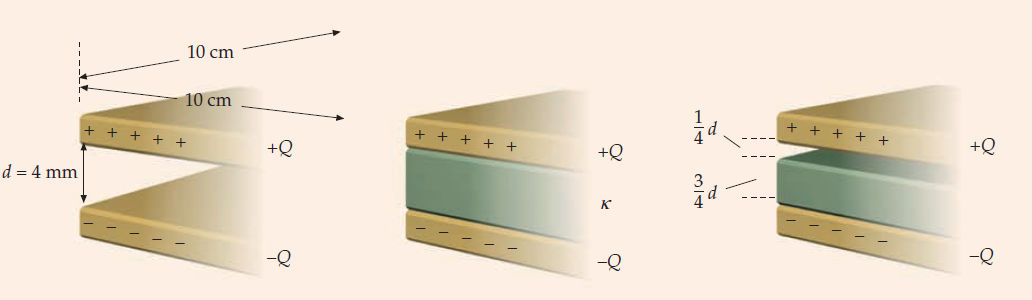
\includegraphics[scale=0.6]{qfig6-20220919-2.png}
  \caption{\textbf{문제 1}}
  \label{fig:1}
\end{figure}
\begin{itemize}
\item[(가)] 우선 평행판 축전기의 전기용량을 구하여라. 
\item[(나)] 유전물질이 들어있지 않을 때 전기용량은 얼마인가?  
\item[(다)] 만약에 양 판 사이에 유전물질이 가득 차 있다면, 이 축전기의
  전기용량은 얼마인가? 
\item[(라)] 이 두 판 사이에 크기가 $10\,\mathrm{cm}\times
  10\,\mathrm{cm}\times 3.0\,\mathrm{mm}$인 유전물질을 넣었다. 이
  축전기의 전기용량은 얼마인가? 
\end{itemize}
여기서 $\epsilon_0=8.85$ pF/m이다. 
\newpage
{\color{gray} [문제 풀이 쪽]}
\newpage

\noindent {\bf 문제 2 [20pt].} 100 W 전구를 120 V 전원에 꽂았다.
\begin{itemize}
\item[(가)] 전구를 계속해서 켜두려면, 31일 동안의 비용은 얼마인가?
  전기에너지의 가격은 60 원 / $\mathrm{kW\cdot h}$라고 가정한다.
\item[(나)] 전구의 저항은 얼마인가?
\item[(다)] 전구에 흐르는 전류는 얼마인가? 
\end{itemize}

\newpage
{\color{gray} [문제 풀이 쪽]}
\newpage

\noindent {\bf 문제 3 [20pt].} 
\begin{figure}[htp]
  \centering
  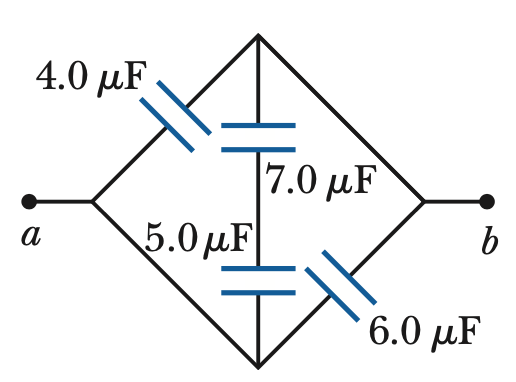
\includegraphics[scale=0.5]{qfig7-1.png}
  \caption{\textbf{문제 3}}
  \label{fig:3}
\end{figure}
그림~\ref{fig:3}에 주어진 $a$와 $b$ 사이에 연결되어 있는 이 축전기들의
등가 전기용량을 구하여라.  
\newpage
{\color{gray} [문제 풀이 쪽]}
\newpage

\noindent {\bf 문제 4 [20pt].} 
가벼운 전기자동차가 있다. 이 차는 12.0 V의 배터리를 직렬로 연결해서
힘을 얻는다. 이 각각의 배터리 내부 저항은 무시할 수 있다. 각각의
배터리는 다시 충전하기 전까지 $160\,\mathrm{A\cdot h}$의 전하를
자동차에 전달한다. 이 자동차가 80.0 km/h의 속력으로 갈 때 이 자동차가
맏는 공기 저항과 구름마찰력(rolling friction)은 1.20 kN이다. 
\begin{itemize}
\item[(가)] 만약에 자동차가 80.0 km/h로 가고 있을 때 전기 모터가
  자동차에 전해주는 최소 일률은 얼마인가?
\item[(나)] 충전이 필요하기 전까지 이 직렬로 연결되어 있는 열 개의
  배터리가 전달하는 총전하는 얼마인가?(coulomb의 단위를 써서
  나타내어라.) 
\item[(다)] 재충전이 필요하기 전까지 열 개의 배터리가 전달하는 총
  전기에너지는 얼마인가? 
\item[(라)] 배터리가 재충전을 필요로 하기 전까지 이 자동차는 얼마나
  멀리 갈 수 있는가?(자동차의 속력은 80.0 km/h로 일정하다.)
\item[(마)] 배터리를 충전하는 데 1 kW-h 당 100원이 든다면, 킬로미터 당
  전기료는 얼마가 필요한가? 
\end{itemize}

\newpage
{\color{gray} [문제 풀이 쪽]}
\newpage

\end{document}